Como enunciamos en la explicaci\'on de nuestro algoritmo, el mismo va chequeando en cada paso si existe alg\'un gimnasio capaz de ser vencido y si existe buscar cual es el m\'as cercano de estos a ser vencidos, por lo tanto existir\'an casos en los cuales la soluci\'on obtenida para los mismos sea la \'optima pero para algunos no lo ser\'a.

Con respecto a las soluciones obtenidas y las \'optimas dado nuestro algoritmo mostraremos las familias de casos en las cuales la soluci\'on obtenida para el greedy es la \'optima:

\begin{enumerate}
\item No se obtiene soluci\'on por no haber las pokeparadas necesarias para ganar en todos los gimnasios.
\item No se obtiene soluci\'on ya que la capacidad de la mochila no puede contener las pociones necesarias para vencer a un cierto gimnasio.
\item Todos los gimnasios sin necesidad de pociones para ser vencidos.
\item Las pokeparadas y los gimnasios se reciben en orden de la forma en la cual exista una pokeparada puntual para ir a cada gimnasio
\end{enumerate}

A continuaci\'on se mostraran las familias en detalle:\\

\begin{center}
\textbf{Familia 1 y 2}
\end{center}

Ambas familias devolveran -1 ya que como se explico anteriomente tanto el greedy como el exacto presentan podas para estos casos sin soluci\'on por lo tanto su tiempo de ejecuci\'on tambi\'en ser\'a id\'entico.

\vspace*{0.3cm} \vspace*{0.3cm}
  \begin{center}
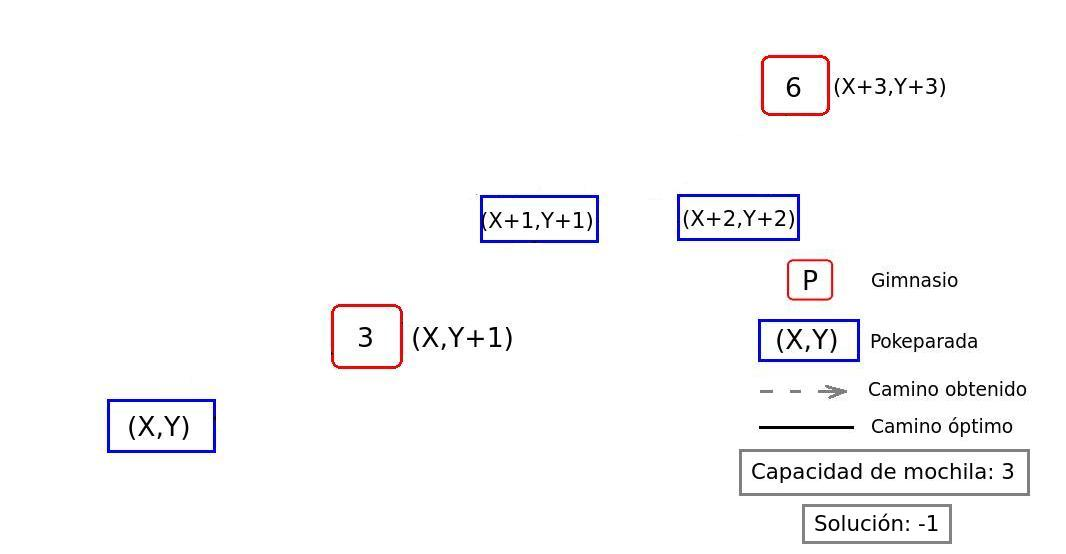
\includegraphics[scale=0.60]{./EJ2/sinSolucion.jpeg}
\\{\textit{Ejemplo 2.1 La soluci\'on obtenida es la \'optima: -1 (Sin soluci\'on)}}
  \end{center}
  \vspace*{0.3cm}
  
  \vspace*{0.3cm} \vspace*{0.3cm}
  \begin{center}
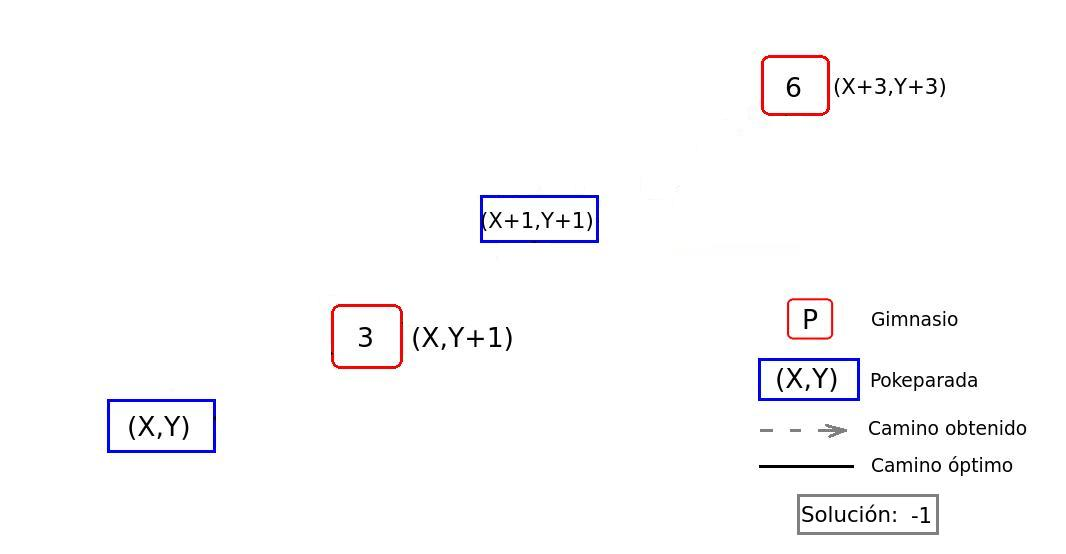
\includegraphics[scale=0.60]{./EJ2/sinSolucion1.jpeg}
\\{\textit{Ejemplo 2.2 La soluci\'on obtenida es la \'optima -1 (Sin soluci\'on)}}
  \end{center}
  \vspace*{0.3cm}


/---> FALTA LA MEDICION CON EL GRAFICO DE TIEMPOS

\begin{center}
\textbf{Familia 3}
\end{center}

En este caso, como nuestro greedy chequea si hay alg\'un gimnasio a ser vencido con la cantidad de pociones que se tienen en el momento (se inicia con 0), y como todos necesitan 0, recorre los gimnasios sin necesidad de pasar por las pokeparadas, obteniendo la mejor soluci\'on posible.

  \vspace*{0.3cm} \vspace*{0.3cm}
  \begin{center}
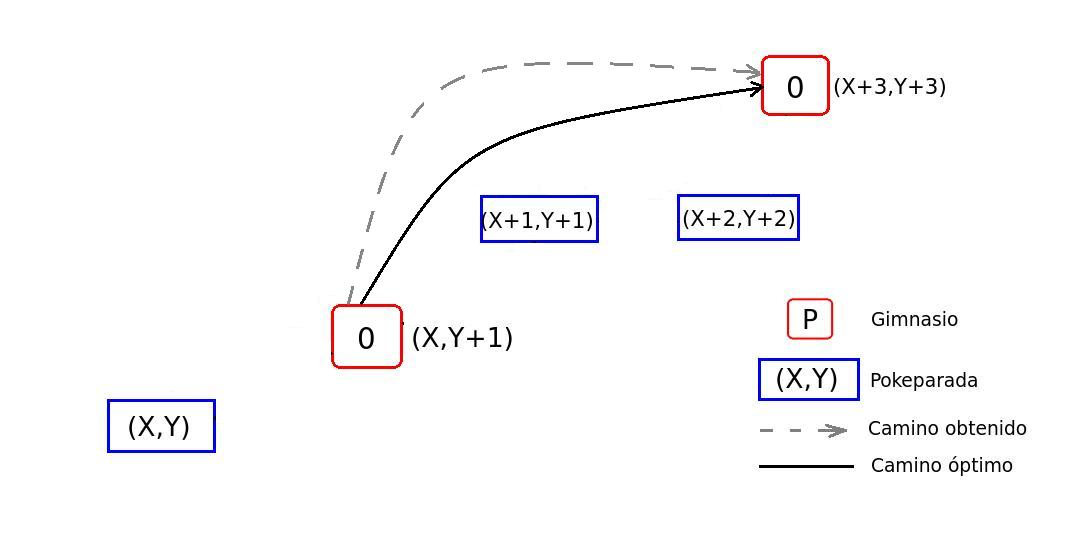
\includegraphics[scale=0.60]{./EJ2/gym0.jpeg}
\\{\textit{Ejemplo 2.3 La soluci\'on obtenida es la \'optima (Devuelve el camino optimo de recorrer todos los gyms)}}
  \end{center}
  \vspace*{0.3cm}


\begin{center}
\textbf{Familia 4}
\end{center}

Se obtendr\'a la soluci\'on \'optima ya que, se reciben primero pokeparadas para vencer a un gimnasio cerca de ellas y luego m\'as pokeparadas para vencer a otros gimnasios que se encuentren cerca de estas \'ultimas, se mostrar\'a a continuaci\'on un dibujo que ejemplifica lo dicho:

\vspace*{0.3cm} \vspace*{0.3cm}
  \begin{center}
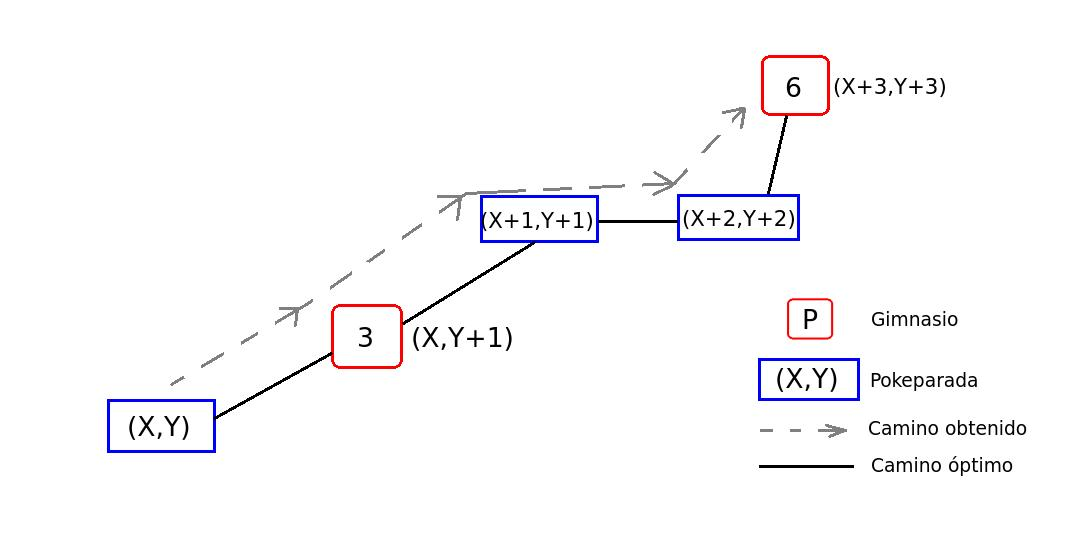
\includegraphics[scale=0.60]{./EJ2/optima.jpeg}
\\{\textit{Ejemplo 2.4 - La soluci\'on obtenida es la \'optima}}
  \end{center}
  \vspace*{0.3cm}

En cambio, no se obtendr\'a una soluci\'on \'optima cuando en vez de juntar una determinada cantidad de poder para vencer varios gimnasios consecutivos, el algoritmo decida ir a una pokeparada y luego a un gimnasio a derrotarlo, para luego repetir esta secuencia.

Con motivo de lo enunciado pudimos elaborar ciertas familias de casos en las cuales la solucion obtenida no es la \'optima, las cuales enunciaremos a continuaci\'on y daremos una explicacion en detalle de cada una:

\begin{enumerate}
\item Elección de gimansios con cero poder 
\item Anillos de pokeparadas y gimnasios
\item Entrada fuera de orden (orden diferente para lograr el óptimo)
\item Movida segura
\end{enumerate}

\begin{center}
Familia sin soluci\'on \'optima n\'umero 1
\end{center}

Este estilo de familia se elabora de la forma en la cual existan gimnasios que no necesiten pociones para ser vencidos y otros que si. Nuestro algoritmo como por cada iteraci\'on chequea si puede elegir un gimnasio que se encuentre a una distancia m\'inima en relaci\'on a los demas, y adem\'as corrobora si posee las pociones necesarias para vencerlo, decide inicialmente ir a vencer a los gimnasios que posean cero poder, lo cual puede no ser \'optimo para el resultado final.

Debido al poder de computo, el algoritmo exacto solo puede tomar hasta 20 elementos, mientras que el goloso puede tomar una mayor cantidad de elementos. Es por esto que se realizaron las comparaciones con la cantidad de elementos soportadas por el exacto.

\vspace*{0.3cm} \vspace*{0.3cm}
  \begin{center}
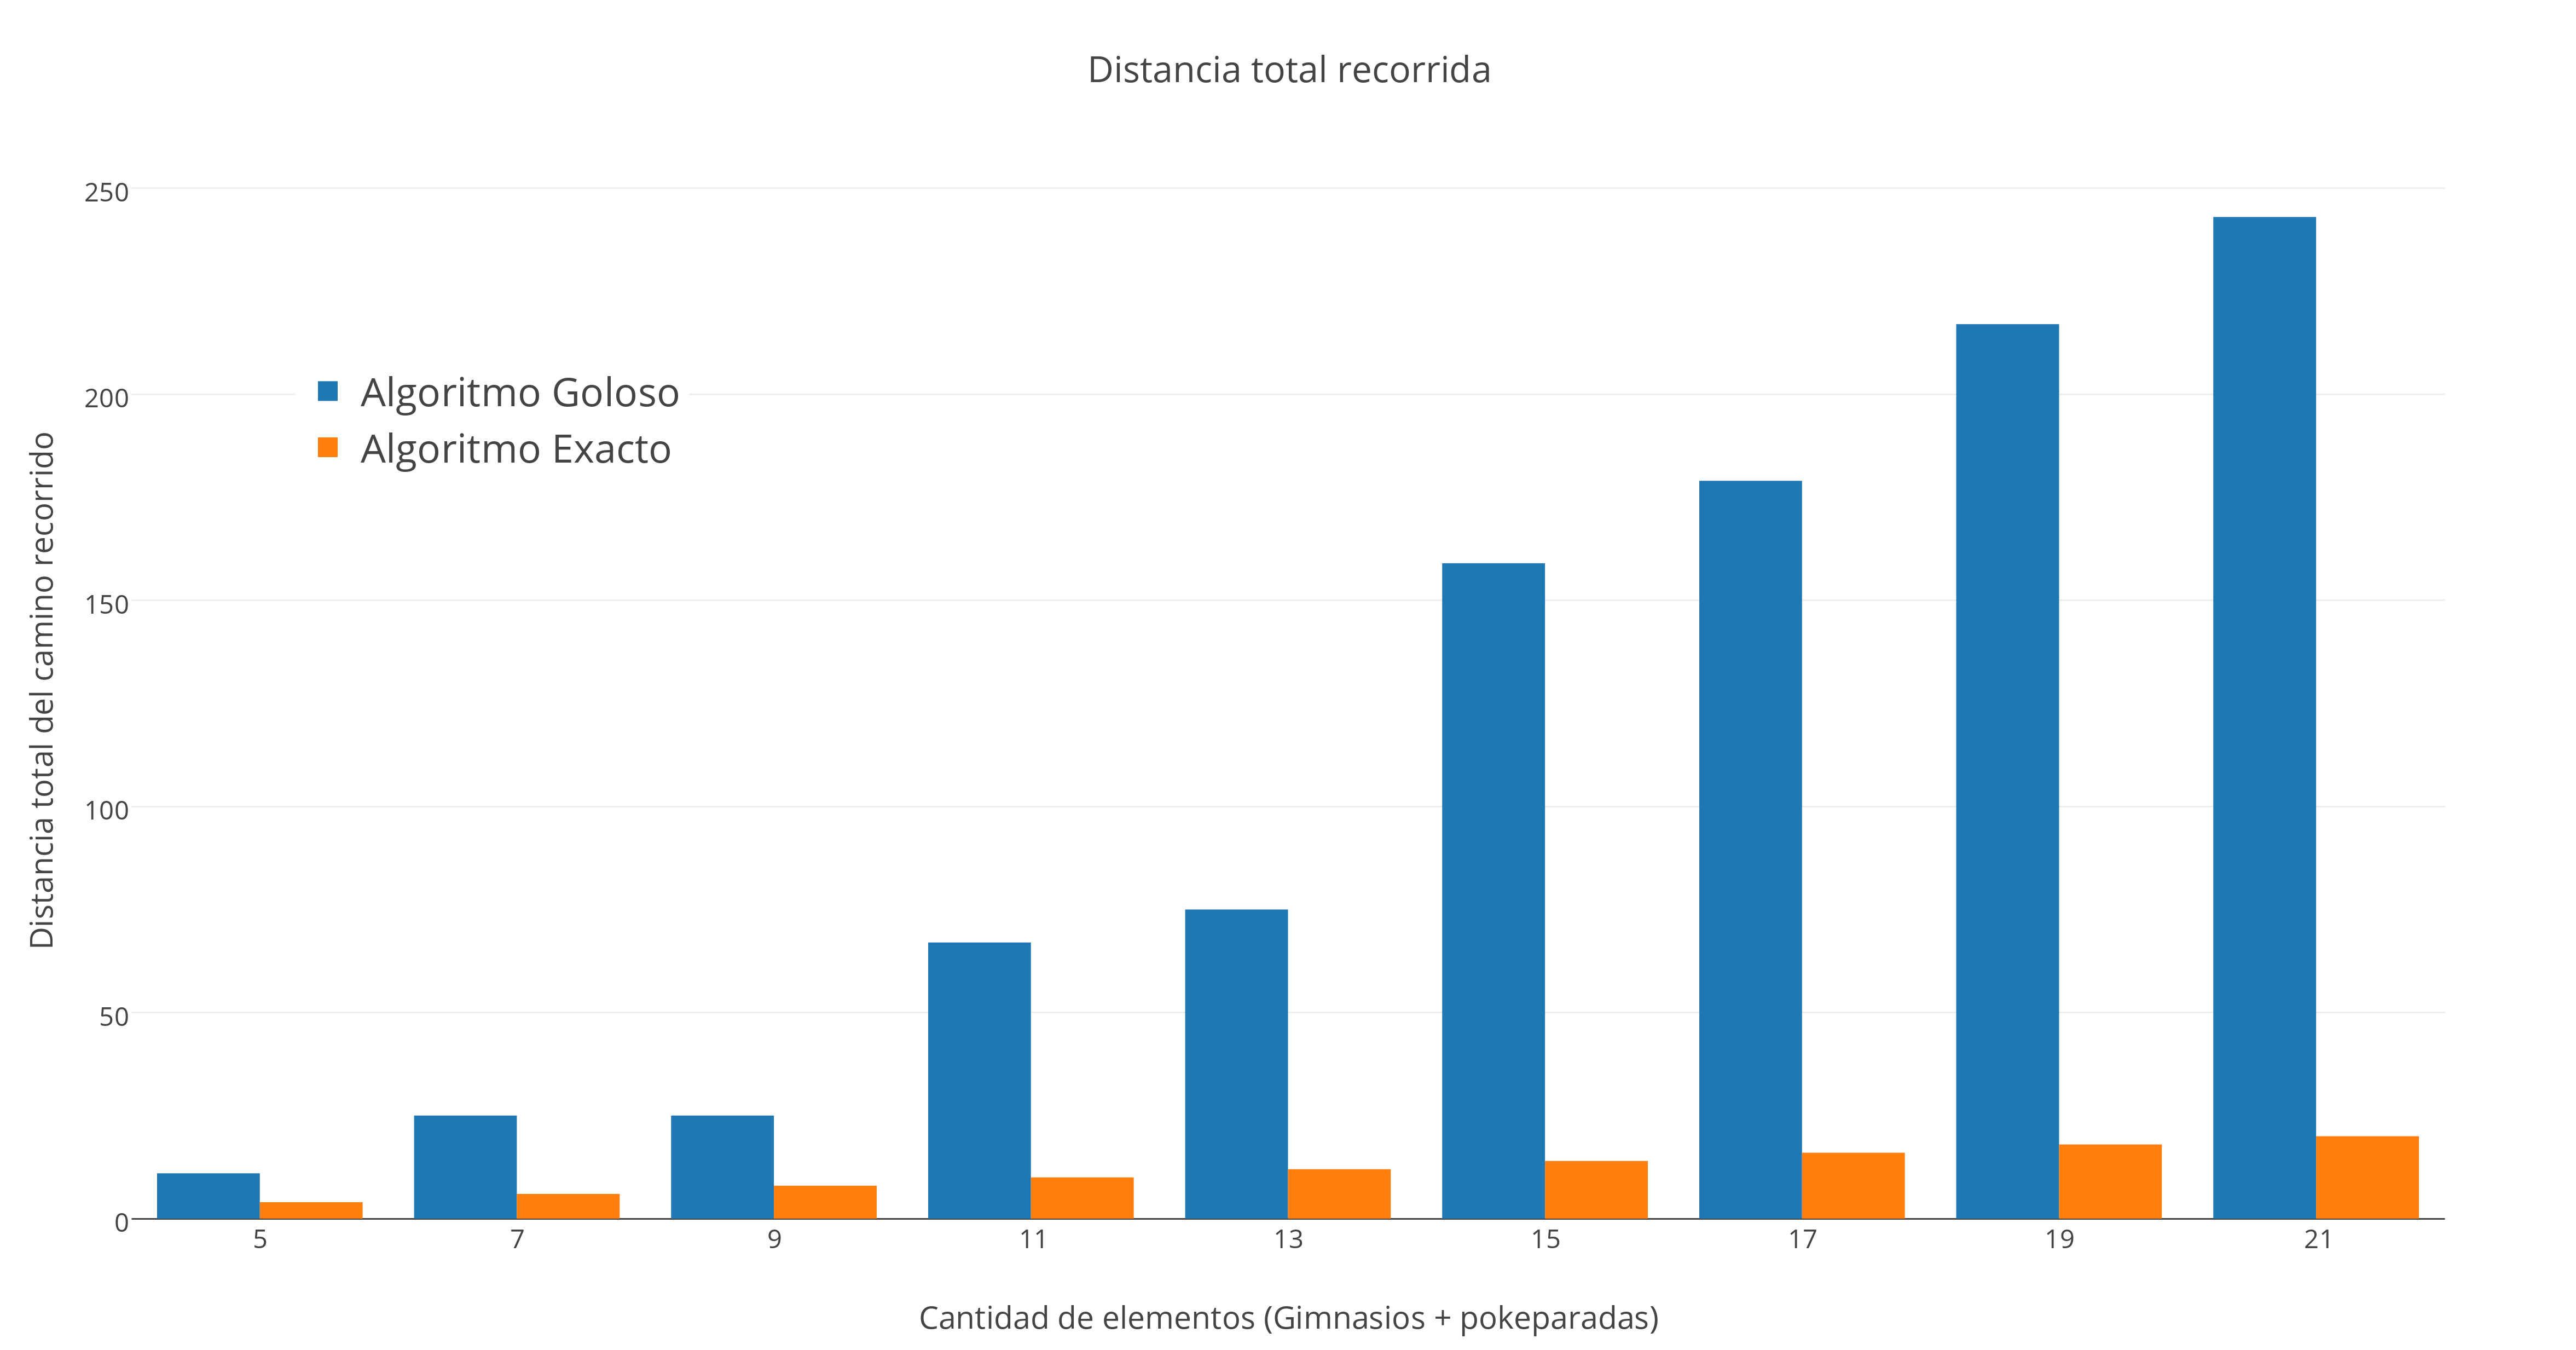
\includegraphics[scale=0.5]{./EJ2/algungym0.png}
\\{\textit{Ejemplo 2.5 Resultados obtenidos (Camino recorrido total) }}
  \end{center}
  \vspace*{0.3cm}

\vspace*{0.3cm} \vspace*{0.3cm}
  \begin{center}
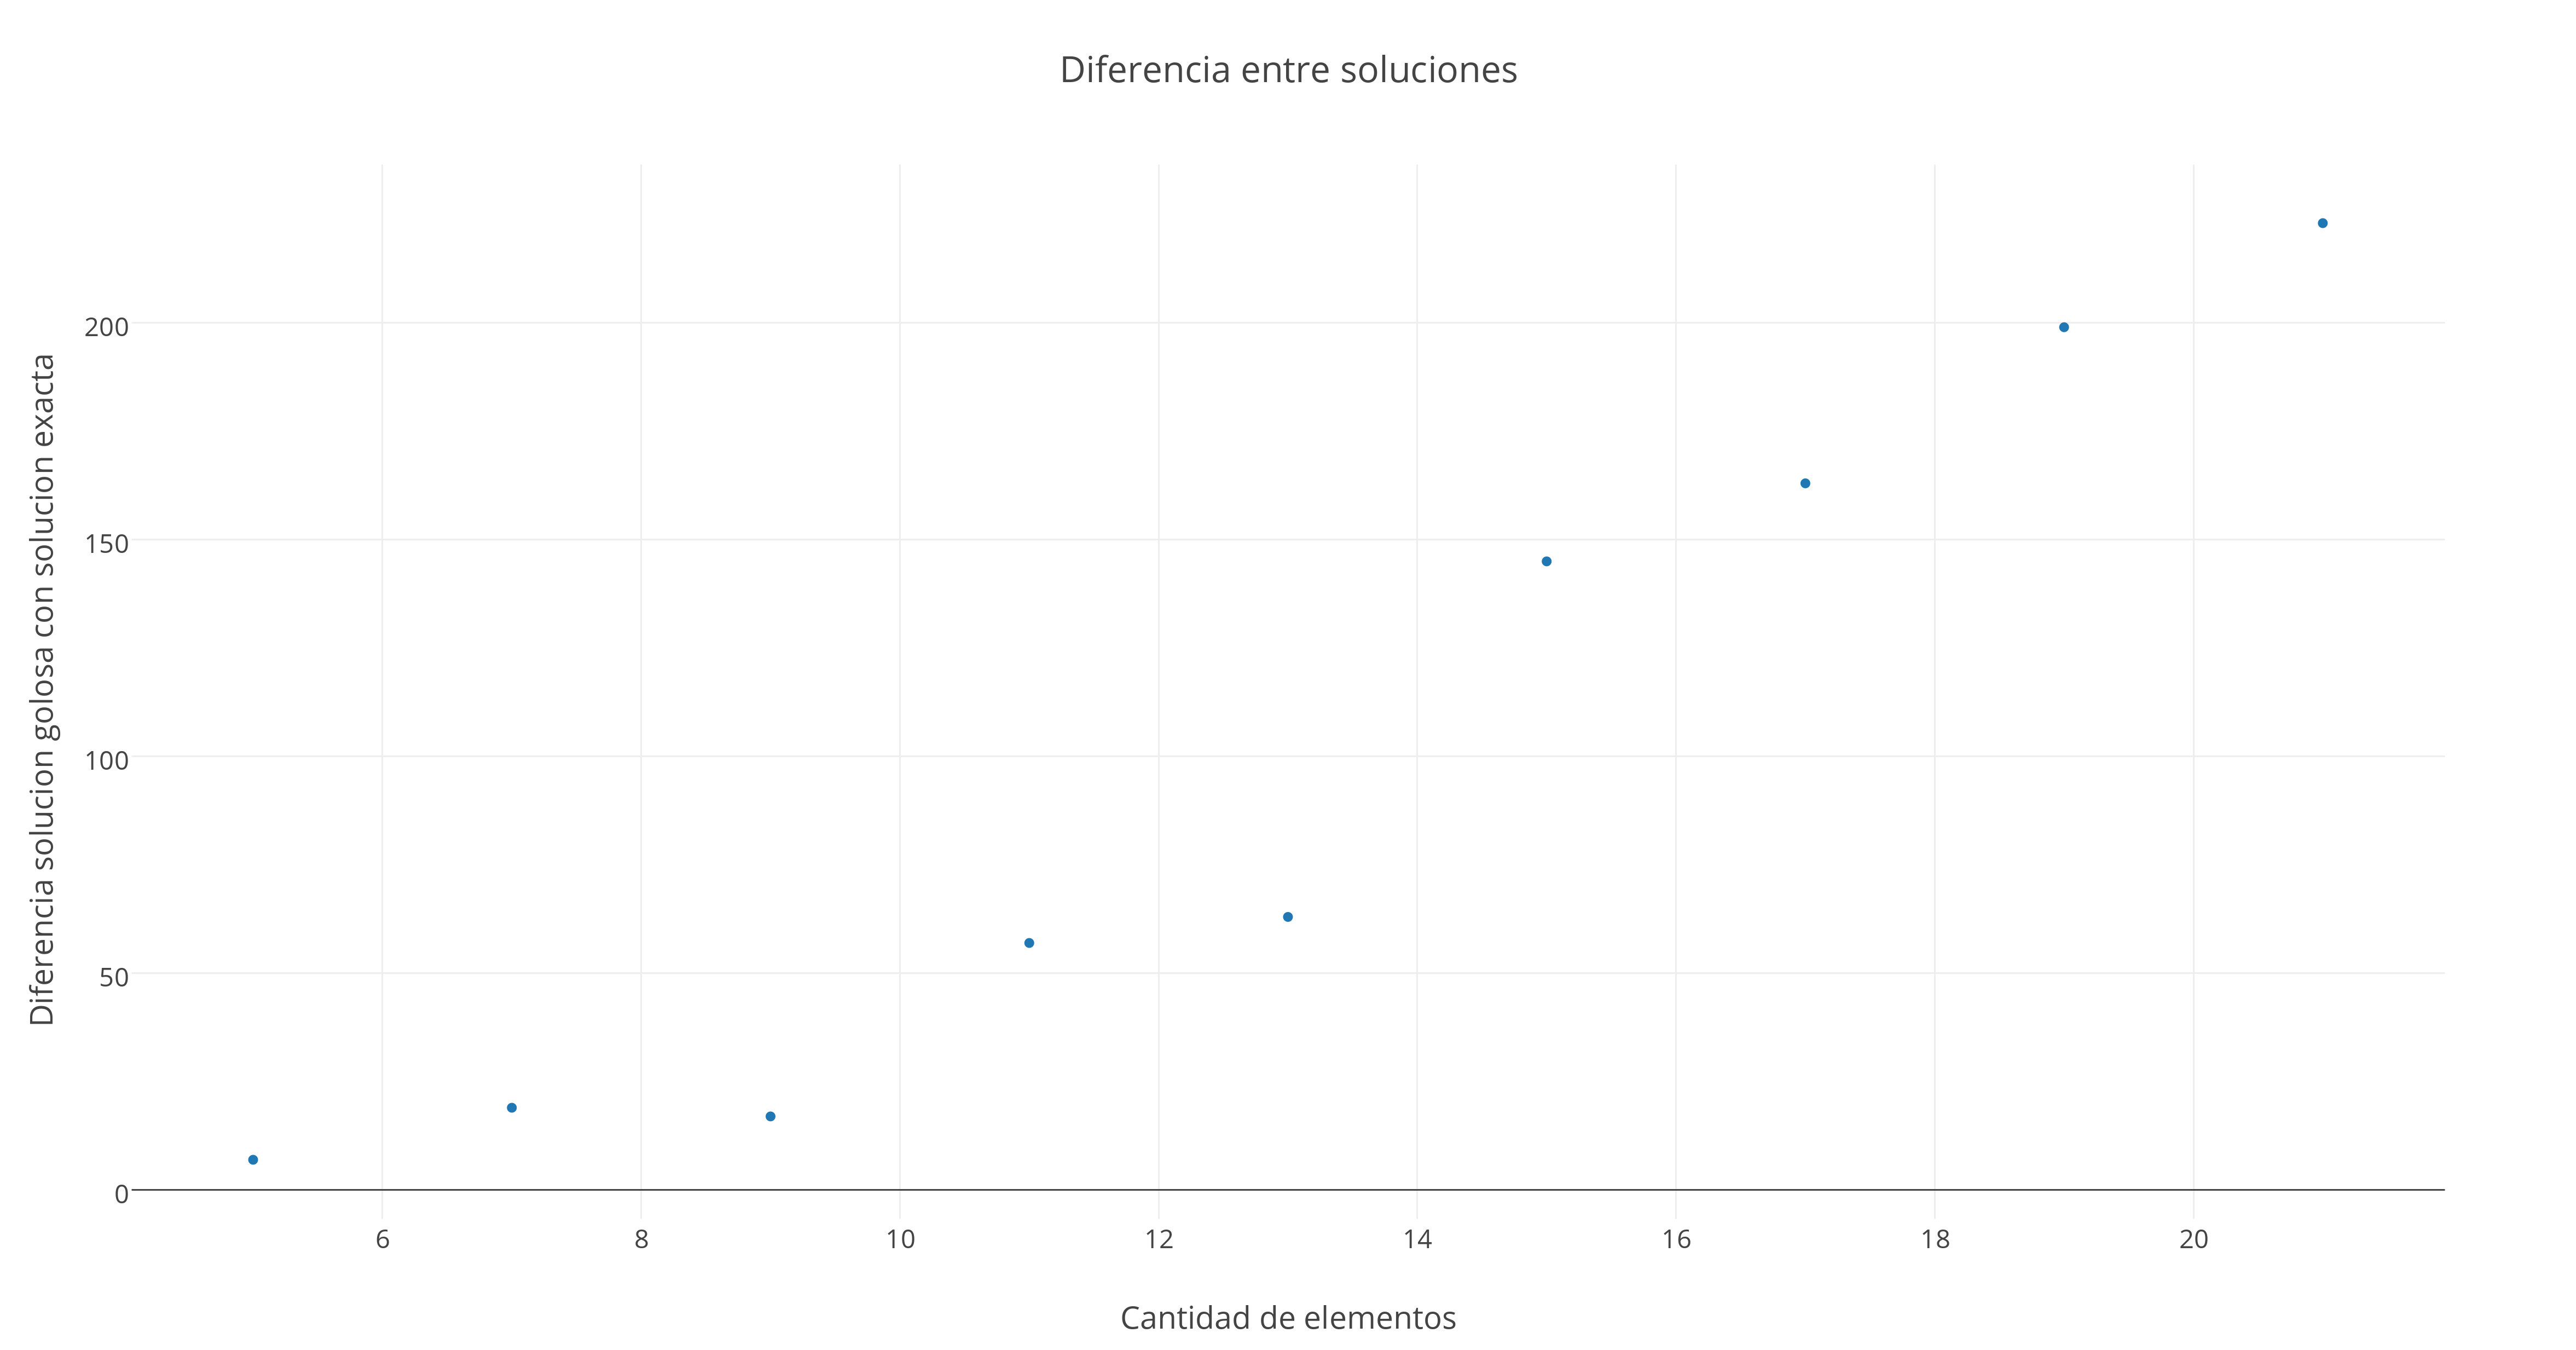
\includegraphics[scale=0.5]{./EJ2/Diferenciagym0.png}
\\{\textit{Ejemplo 2.5 Diferencia resultados obtenidos (Camino recorrido total) }}
  \end{center}
  \vspace*{0.3cm}


\begin{center}
Familia sin soluci\'on \'optima n\'umero 2
\end{center}

Este estilo de familia se elabora de la forma en la cual se tengan todos los gimnasios en ciertas posiciones, donde el conjunto total de estos nos devuelva una forma de anillo, mientras que las pokeparadas presenten la misma forma que los gimnasios a una distancia euclidea id\'entica entre pokeparada-gimnasio. Como mencionamos nuestro algoritmo siempre que puede vencer a alg\'un gimnasio busca cual es el m\'inimo en relaci\'on a la distancia y va a vencerlo, lo cual en este caso puntual ser\'a contraproducente ya que es preferible adquirir m\'as pociones para luego ir a varios gimnasios juntos. (ESTO HABRIA QUE REESCRIBIRLO PORQUE NO QUEDA MUY CLARO)


/----> PONER DIBUJO Y GRAFICO QUE MUESTRE COMO VARIA LA SOLUCION OBTENIDA ENTRE EXACTO Y EL GOLOSO 

\vspace*{0.3cm} \vspace*{0.3cm}
  \begin{center}
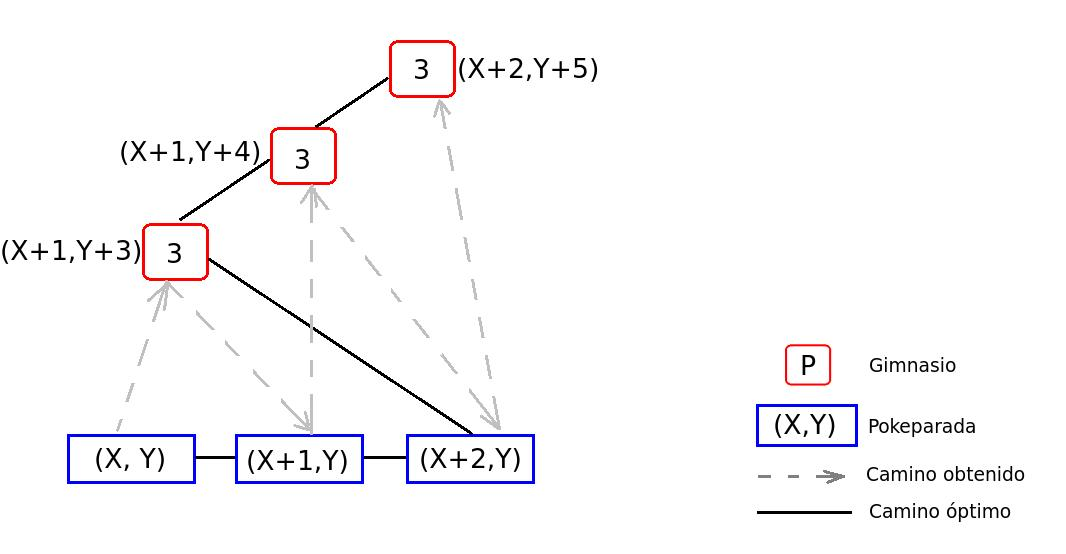
\includegraphics[scale=0.60]{./EJ2/nooptima.jpeg}
\\{\textit{Ejemplo 2.5 La soluci\'on obtenida no es la \'optima}}
  \end{center}
  \vspace*{0.3cm}

Se puede observar en el ejemplo 2.5 como nuestro algorimo va a la primer pokeparada y de ah\'i va a vencer al gimnasio m\'as cercano en vez de ir a la pokeparada que se encuentra inmediatamente consecutiva. Esto lo hace hasta vencer a todos los gimnasios.

\begin{center}
Familia sin soluci\'on \'optima n\'umero 3
\end{center}

Este estilo de familia presenta a los gimnasios y pokeparadas desordenados en referencia a las posiciones, es decir, es decir para ganar a cierto gimnasio es necesario pasar por una cantidad puntual de pokeparadas las cuales estan de un lado y del otro de dicho gimnasio.
(VER DE ESCRIBIR ESTO MAS EN DETALLE)

/----> PONER GRAFICO QUE MUESTRE COMO VARIA LA SOLUCION OBTENIDA ENTRE EXACTO Y EL GOLOSO 



\vspace*{0.3cm} \vspace*{0.3cm}
  \begin{center}
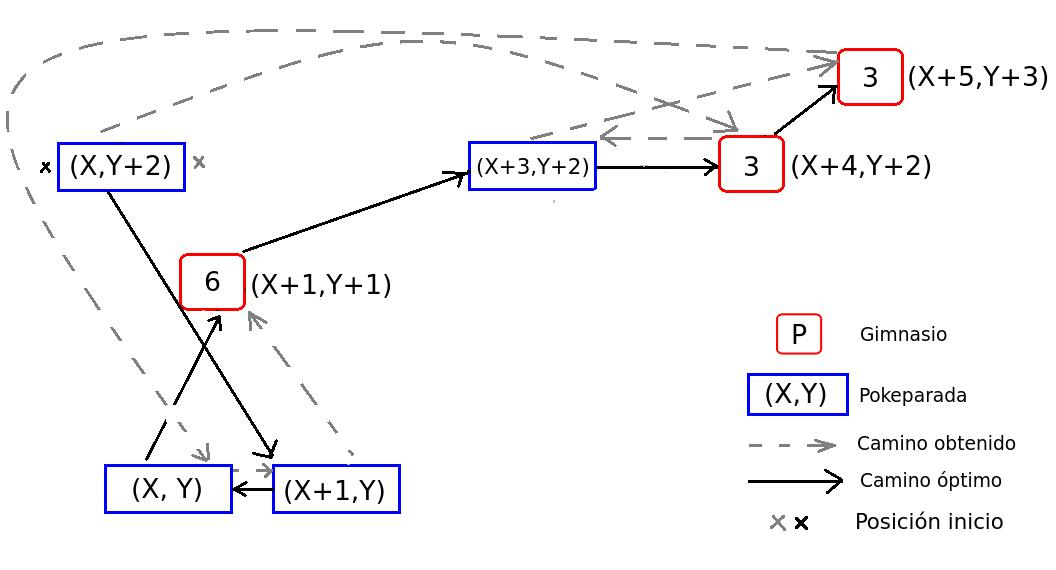
\includegraphics[scale=0.60]{./EJ2/nooptima2.jpeg}
\\{\textit{Ejemplo 2.5 La soluci\'on obtenida no es la \'optima}}
  \end{center}
  \vspace*{0.3cm}
  
  
  
Por \'ultimo, la familia sin soluci\'on \'optima n\'umero 4 estar\'a formada por 2 conjuntos de gimnasios y otro de pokeparadas donde habr\'a un conjunto de gimnasios con poder 6 que se encontrar\'a m\'as cerca a las pokeparadas que el otro conjunto el cual tendr\'a poder 3. Nuestro algoritmo como mencionamos, ir\'a a una pokeparada y luego a alg\'un gimnasio con poder 3 en ves de ir a otra pokeparada para primero ganar en los gimnasios de 6.

/----> PONER GRAFICO QUE MUESTRE COMO VARIA LA SOLUCION OBTENIDA ENTRE EXACTO Y EL GOLOSO 

\vspace*{0.3cm} \vspace*{0.3cm}
  \begin{center}
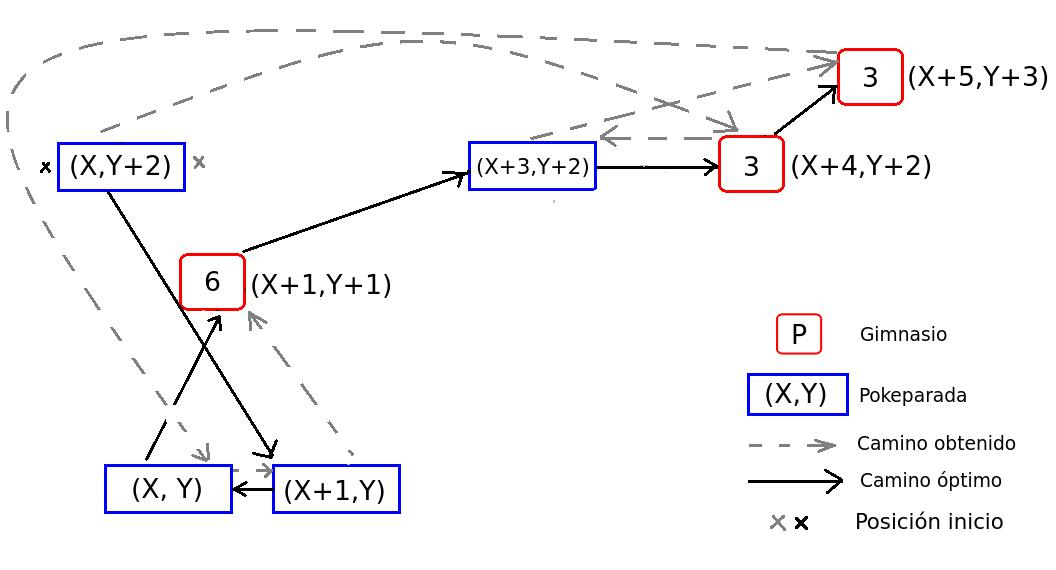
\includegraphics[scale=0.60]{./EJ2/nooptima2.jpeg}
\\{\textit{Ejemplo 2.6 La soluci\'on obtenida no es la \'optima}}
  \end{center}
  \vspace*{0.3cm}


En conclusi\'on, la soluci\'on obtenida distará tanto de la óptima como la cantidad de veces que el algoritmo recorra una pokeparada y luego un gimnasio a vencerlo, sin importar si lo más optimo era pasar primero por las pokeparadas juntando poder y luego visitar varios gimnasios consecutivamente venciendolos a todos.
El peor caso será cuando el mapa sea un anillo de pokeparadas con un anillo interno o externo de gimnasios. 
El algoritmo iniciará en una pokeparada, luego irá a ganar a un gimansio con distancia mínima dentro de los gimansios no visitados, y siguiendo este recorrido, volverá a una pokeparada que se encuentre a una distancia menor de la pokeparada previa.\\



